\documentclass[border=10pt]{standalone}

\usepackage{tikz}
\usepackage{tikzsymbols}
\usetikzlibrary{calc,patterns,shapes.geometric}

\def\centerarc[#1](#2)(#3:#4:#5){\draw[#1] ($(#2)+({#5*cos(#3)},{#5*sin(#3)})$) arc (#3:#4:#5);}

\begin{document}
	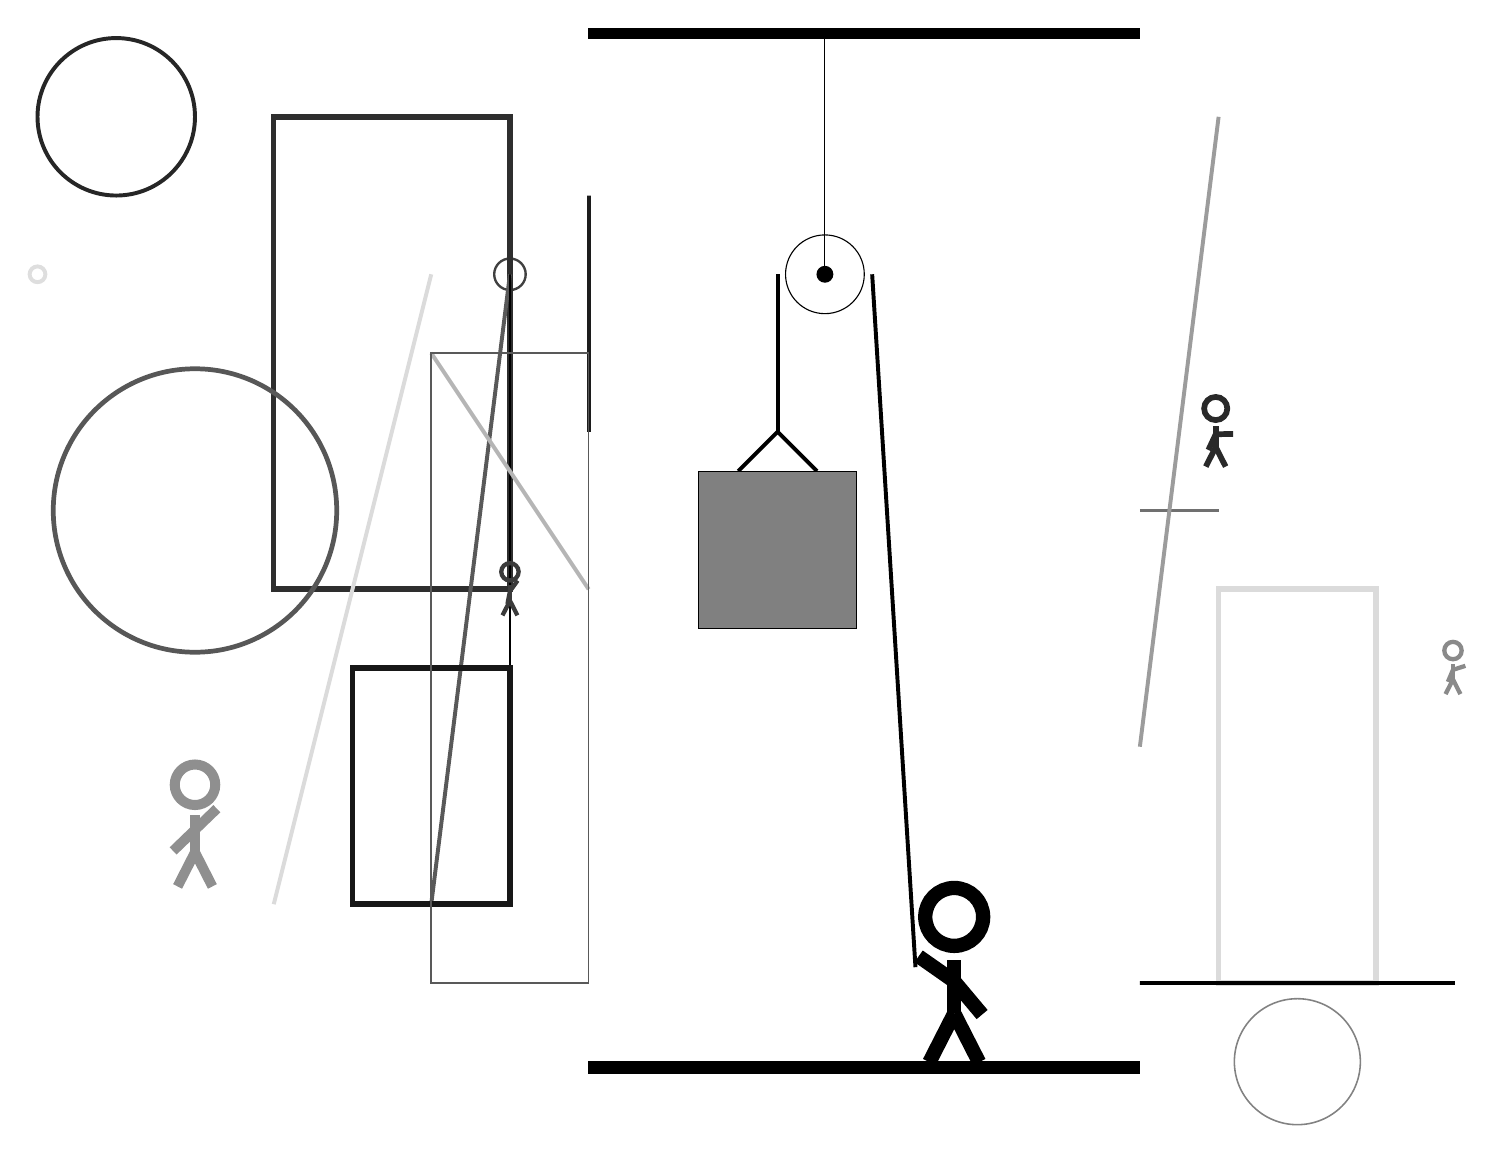
\begin{tikzpicture}
		%%%%% START %%%%%
		
		\draw[fill=black] (-2, 10) rectangle (5, 10.125);
		
		\draw (1, 7) circle (0.5);
		\draw[fill=black] (1, 7) circle (0.1);
		\draw (1, 10) -- (1, 7);
		
		\draw[line width=0.5mm] (-0.1, 4.5) -- (0.4, 5.0) -- (0.9, 4.5);
		\draw[fill=black!50] (-0.6, 4.5) rectangle (1.4, 2.5);
		
		\draw[line width=0.5mm] (0.4, 7) -- (0.4, 5.0);
		\centerarc[line width=0.5mm](1, 7)(0:180:0.6);
		\draw[line width=0.5mm](1.6, 7) -- (2.15, -1.8);
		
		\node at (2.6, -1.9) {\Strichmaxerl[10][-35][-50]};
		
		\draw[line width=0.5mm, color=black!56](5, 4) -- (6, 4);
		
		\node[line width=0.5mm, color=black!44] at (-7, 0) {\Strichmaxerl[7][44][44]};
		\draw [line width=0.3mm, color=black!75](-3, 7) circle (0.2);
		\draw[line width=0.7mm, color=black!82] (-3, 9) rectangle (-6, 3);
		
		\draw [line width=0.5mm, color=black!13](-9, 7) circle (0.1);
		\draw[line width=0.5mm, color=black!65](-3, 7) -- (-4, -1);
		\node[line width=0.5mm, color=black!46] at (9, 2) {\Strichmaxerl[3][67][18]};
		\node[line width=0.7mm, color=black!84] at (6, 5) {\Strichmaxerl[4][65][1]};
		\draw[line width=0.3mm, color=black!100] (-3, 7) rectangle (-3, 2);
		\draw[line width=0.5mm, color=black!89] (-2, 5) rectangle (-2, 8);
		\draw[line width=0.7mm, color=black!91] (-3, -1) rectangle (-5, 2);
		\draw[line width=0.5mm, color=black!29](-4, 6) -- (-2, 3);
		\draw[line width=0.5mm, color=black!14](-4, 7) -- (-6, -1);
		\node[line width=0.2mm, color=black!77] at (-3, 3) {\Strichmaxerl[3][79][54]};
		\draw[line width=0.7mm, color=black!14] (6, 3) rectangle (8, -2);
		\draw [line width=0.5mm, color=black!85](-8, 9) circle (1.0);
		
		\draw [line width=0.2mm, color=black!49](7, -3) circle (0.8);
		\draw[line width=0.5mm, color=black!39](6, 9) -- (5, 1);
		\draw [line width=0.6mm, color=black!66](-7, 4) circle (1.8);
		\draw[line width=0.5mm, color=black!100] (5, -2) rectangle (9, -2);
		\draw[line width=0.2mm, color=black!65] (-2, 6) rectangle (-4, -2);
		
		\draw[fill=black] (-2, -3) rectangle (5, -3.15);
		
		%%%%% END %%%%%
	\end{tikzpicture}
\end{document}